\documentclass[10 pt]{article}
\usepackage[margin=0.5 in]{geometry}
\usepackage[utf8]{inputenc}
\usepackage{tikz}
\usetikzlibrary{arrows}
\usepackage{tabu}
\usepackage{color}
\usepackage{xcolor}
\usepackage{listings}
\usepackage{enumitem}

\usepackage{multicol}


\setlength{\columnsep}{1cm} 

\title{\textbf {Estructuras de Datos 2 - ST0247\\Examen Parcial 1 - Jueves (032)
}}
\author{Nombre ..............................\\
		Departamento de Informática y Sistemas\\
		Universidad EAFIT\\}
\date{21 de Marzo de 2019}
\begin{document}
\lstdefinestyle{customc}{
	language=Java, 
	numbers=left, 
	showspaces=false,
    showstringspaces=false, 
    tabsize=2, 
    breaklines=true,
    xleftmargin=5.0ex,
}
\lstset{escapechar=@,style=customc, numbers=left, stepnumber = 1} 
\maketitle

\textbf{En las preguntas de selección múltiple, una respuesta incorrecta tendrá
una deducción de 0.2 puntos en la nota final. Si dejas la pregunta sin
responder, la nota será de 0.0. Si no conoces la respuesta, no adivines.}

\begin{multicols}{2}

	\section{BFS y Grafos (20\%)}
	Como bien sabes, un \emph{árbol} es un grafo no dirigido con $n$ vértices y $n - 1$ artistas donde el peso de cada arista es 1. Considera un árbol con raíz $v$. Sabemos que $d_i$, usando algoritmo de \emph{búsqueda primero en amplitud} (en Inglés, BFS), es la distancia más corta  del nodo $v$ al nodo $i$. En este ejercicio, vamos a encontrar el \textit{diámetro} de un árbol de $n$ nodos. El diámetro de un árbol se define como el número máximo de aristas del camino más corto entre cualesquiera dos vértices del árbol. Como un ejemplo, en el siguiente árbol, se resalta su diámetro, el cual es de $4$.
	\\
	\begin{center}
		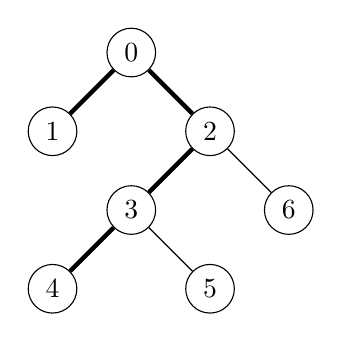
\begin{tikzpicture}	
		\tikzset{vertex/.style = {shape=circle,draw,minimum size=1.5em}}
		\tikzset{edge/.style = {-,> = latex'}}
		\node[vertex] (0) at (0, 0)  {0};
		\node[vertex] (1) at (-1, -1) {1};
		\node[vertex] (2) at (1, -1) {2};
		\node[vertex] (3) at (0, -2) {3};
		\node[vertex] (4) at (-1, -3) {4};
		\node[vertex] (5) at (1, -3) {5};
		\node[vertex] (6) at (2, -2) {6};
		%edges
		\draw[-, ultra thick] (0) to (1);
		\draw[-, ultra thick] (0) to (2);
		\draw[-, ultra thick] (2) to (3);
		\draw[-, ultra thick] (3) to (4);
		\draw[edge] (3) to (5);
		\draw[edge] (2) to (6);
		\end{tikzpicture}
	\end{center}

La siguiente es la implementación del algoritmo de BFS para calcular las
	distancias más cortas del nodo $v$ a todos los demás nodos de un árbol
	{\footnotesize
	\begin{lstlisting}
	//Retorna di: las distancias mas cortas
	// del nodo v al nodo i
	int[] bfs(ArrayList<Integer>[] g, int v) {
	  int[] d = new int[g.length];
	  Arrays.fill(d, Integer.MAX_VALUE);
	  d[v] = 0;
	  Queue<Integer> q;
	  q = new LinkedList<Integer>();
	  q.add(v);
	  while(!q.isEmpty()){
	  	int s = q.poll();
	  	Iterator<Integer> i=g[s].listIterator();
	  	while(i.hasNext()){
	  	  int n = i.next();
	  	  if(d[s] + 1 < d[n]){
	  	    d[n] = d[s] + 1;
	  	    q.add(n);
	  	  }
	  	}
	  }
	  return d;
	}
	\end{lstlisting}
	}

	Para encontrar el diámetro de un árbol se puede usar el siguiente algoritmo:
	\begin{itemize}
		\item Tomar un vértice $v$ como raíz del árbol $g$ y encontrar $d_i$, para todo $i$, usando \texttt{bfs(g, v)}.
		\item Encontrar un vértice $u$ como nodo inicial tal que $d_u \geq d_t$ para todo $t$. Sea $f_i$ la distancia más corta del nodo $u$ a cualquier nodo $i$ del árbol, el diámetro del árbol es $\max\limits_i{f_i}$
	\end{itemize}
	{\footnotesize
	\begin{lstlisting}
	int diametro(ArrayList<Integer> g[]){
	  int v, u, w;
	  v = u = w = 0;
	  int[] d = bfs(g, v);
	  int n = d.length;
	  for(int i = 0; i < n; ++i)
	    if( ............ ) u = i;
	  int[] f = bfs(g, u);
	  for(int i = 0; i < n; ++i)
	    if( .......... ) w = i;
	  return f[w];
	}
	\end{lstlisting}
	}
	\begin{enumerate}[label=\alph*]
		\item (10\%) ¿Cuál es la complejidad asintótica, en el peor de los casos, del algoritmo anterior?
		% Respuesta O(n)
		\begin{enumerate}[label=\roman*]
			\item $O(n)$
			\item $O(n^2)$
			\item $O(n \log n)$
			\item $O(n \times \sqrt{n})$
		\end{enumerate}
		% Respuesta: d[i] > d[u], f[i] > f[w]
		\item (10\%) Complete las líneas 7, 13 ............, ............
	\end{enumerate}



	\section{Backtracking (20\%)}
	Te entregan una cadena de caracteres $s$ y un entero $n$, $n \geq |s|$. Necesitamos contar todas las posibles cadenas de caracteres de tamaño a lo sumo $n$, que contienen \textbf{al menos una vez} cada uno de los caracteres de $s$. Las cadenas generadas sólo pueden contener los caracteres de $s$. Como algunos ejemplos: 
	{\footnotesize
	\begin{itemize}[noitemsep]
		\item $s = ``a''$, $n = 2$. Respuesta: $2$. ``a'', ``aa''
		\item $s = ``ab''$, $n = 2$. Respuesta: $2$.  ``ab'', ``ba''
		\item $s = ``ab''$, $n = 3$. Respuesta: $8$.  ``aab'', ``ab'', ``aba'', ``abb'', ``ba'', ``baa'', ``bab'', ``bba''.
		\item $s = ``abc''$, $n = 4$. Respuesta: $42$.
	\end{itemize}

	\textbf{Nota:} \texttt{s.toCharArray()} convierte una cadena de caracteres en un arreglo de caracteres, \texttt{s.contains(c)} verifica si
	un caracter está dentro de una cadena de caracteres o no, y \texttt{s.length()} retorna la longitud de una cadena.
	}
	{\footnotesize
	\begin{lstlisting}
	//s: Cadena dada
	//n: Numero dado
	//gen: Cadena generada
	int count(String s,int n,String gen){
	  if(..............) return 0;
	  int res = 0;
	  //gen contiene todos los
	  //caracteres que hay en s? 
	  boolean all_chars = true;
	  for(char ch: s.toCharArray()){
	    if(.....................){
	      all_chars = false;
	    }
	  }
	  if(all_chars){
	    ..................;  
	  }
	  for(char ch: s.toCharArray()){
	    res += count(s, n, gen + ch);
	  }
	  return res;
	}
	\end{lstlisting}
	}
	\begin{enumerate}[label=\alph*]
		%Respuesta: gen.length() > n, gen.indexOf(ch)
		\item (10\%) Complete las líneas 5, 11 .................., ....................
		% Respuesta: res = 1
		\item (10\%) Complete la línea 16 ...................
	\end{enumerate}




	\section{Fuerza Bruta (20\%)}
	Dadas dos cadenas de caracteres $s_1$ y $s_2$, determine si la cadena $s_2$ aparece al menos $k$ veces en la cadena $s_1$. 
	{\footnotesize
	\begin{lstlisting}
	boolean valid(String s1, String s2, int k){
	  int cnt = 0;
	  for(int i=0; i < s1.length();++i){
	    String s = ..........;
	    for(int j = i + 1; j < s2.length(); ++j){
	      if(s.equals(s2)){
	        cnt++;
	      }
	      s += s1.charAt(j);
	    }
	  }
	  return cnt >= k;
	}
	
	\end{lstlisting} 
	}
	%Respuesta: s1[i], O(s1*s2)
	\begin{enumerate}[label=\alph*]
		\item (10\%) Complete la línea 4 ....................
		\item (10\%) ¿Cuál es la complejidad asintótica, para el peor de los casos, del algoritmo anterior?
		\begin{enumerate}[label=\roman*]
			\item $O(|s1| + |s2|)$
			\item $O(|s1| \times |s2|)$
			\item $O(|s1|^2 + |s2|)$
			\item $O(|s1| + |s2|^2)$		
	\end{enumerate}
	\end{enumerate}
	


	\section{Divide y Vencerás (20\%)}
	Dado un arreglo binario ordenado de manera decreciente $a$ (sólo contiene ceros y unos). Determine el número de unos en el arreglo. El tamaño del arreglo es de $n, n \geq 1$ elementos.
	{\footnotesize
	\begin{lstlisting}
	int count(int[] a, int l, int h){
	  if(h >= l){
	    int m = l + (h - l) / 2;
	    if((m==h || a[m+1]==0)&&(a[m]==1)){
	      return m + 1;
	    }
	    if(a[m] ........){
	      return count(a, m + 1, h);
	    }
	    return count(a, l, m - 1);
	  }
      return 0;
	}
	\end{lstlisting}
	}
	\begin{enumerate}[label=\alph*]
		% Respuesta: a[m] == 1
		\item (10\%) Complete la línea 7 .................
	
	(10\%) ¿Cuál es la complejidad asintótica, en el peor de los casos, del algoritmo anterior?
	\begin{enumerate}[label=\roman*]
		% Respuesta: O(log n)
		\item $T(n) = T(n-1) + c$, que es $O(n)$
		\item $T(n) = T(n/2) + cn$, que es $O(n \log n)$
		\item $T(n) = T(n/2) + c$, que es $O(\log n)$
		\item $T(n) = c$, que es $O(1)$
	\end{enumerate}
	\end{enumerate}


\section{Voraces (20\%)}
%http://www.geeksforgeeks.org/graph-coloring-set-2-greedy-algorithm/
El problema de colorear los vértices de un grafo sirve, por ejemplo, para encontrar las jaulas de un zoológico. 
El problema es el sigueinte: Dado $m$ colores, encontrar una forma de colorear los vértices del grafo de tal
forma que no haya dos vértices adyacentes que usen el mismo color.

Un algoritmo voraz para este problema funciona de la siguiente manera. Primero, se colorea el primer vértice
con el primer color. Segundo, se hace lo siguiente para los $v-1$ vértices restantes: Se intenta colorear el vértice
actual con el color enumerado con el menor valor posible que no haya sido utilizado previamente en un vértice
adyacente a él. Si todos todos los colores disponibles hasta el momento han sido utilizados en vértices
adyacentes al vértice actual, asigna un nuevo color para este vértice.

\textbf{Nota: } Un iterador es un mecanismo que se utiliza en implementación de listas enlazadas para recorrer, en este caso, los vértices adyacentes a un vértice.
Las operaciones siguiente (\texttt{next()}) y hay un siguiente (\texttt{hasNext()}) tienen complejidad $O(1)$.

\end{multicols}

\pagebreak

\begin{lstlisting}
// Asigna colores (empezando en 0) a todos 
// los vertices e imprime la asignacion de colores
void greedyColoring() {
   int result[] = new int[V];
   // Asigna el primer color al primer vertice
   result[0]  = 0;

   // Inicializa los otros v-1 vertices con ??
   for (int u = 1; u < V; u++)
      _________________;  // es decir, u no tiene color

   boolean available[] = new boolean[V];
   for (int cr = 0; cr < V; cr++)
         available[cr] = false;
 
   // Asigna colores a los v-1 vertices
   for (int u = 1; u < V; u++) {
         Iterator<Integer> it = adj[u].iterator() ;
         while (it.hasNext())
         {
                int i = it.next();
                if (result[i] != -1)
                    available[result[i]] = true;
         }
 
         // Encuentra el primer color disponible
         int cr;
         for (cr = 0; cr < V; cr++)
             if (available[cr] == false)
                    break;
 
         result[u] = cr; // Asigna el color encontrado
 
         // Pone los valores en falso para la proxima iteracion
         it = adj[u].iterator() ;
         while (it.hasNext()) {
             int i = it.next();
             if (result[i] != -1)
                available[result[i]] = false;
         }
   }
   for (int u = 0; u < V; u++)
      System.out.println("Vertex " + u + " --->  Color "
                         + result[u]);
}
 \end{lstlisting}


\begin{enumerate}[label=\alph*]


    \item (10\%) ¿Cuál es la complejidad asintótica, para el peor de los casos, para el algoritmo anterior? \\


  O(\_\_\_\_\_\_\_\_\_\_\_\_\_\_\_\_\_)

  \item (10\%) Completa el espacio de código que hace falta en la línea 10, para inicializar los colores \\

\_\_\_\_\_\_\_\_\_\_\_\_\_\_\_\_\_   

  %result[u] = -1
\end{enumerate}

\end{document}